We approach the named entity recognition problem from different perspectives, as a sequence labeling task, a question answering task and a span detection and classification task. In this chapter, we look at all these in detail and compare and contract them with one-another. Primarily, we develop on top of pretrained BERT model. We look at the effect of loss function, tagging schemes, and providing additional semantic information on the overall task. We also study how much guidance the model derives from any additional information fed with the input. Experiments are conducted on multiple datasets and we simultaneously compare our models with previously published state-of-the-art results as well. 

\section{Sequence Labeling}
\begin{definition}
\label{def:seq_labeling}
    Given sentence $\mathcal{S}$ as a $N$-length sequence of tokens, $\mathcal{S} = \langle w_1, w_2 \ldots w_N \rangle$, sequence labeling is the task of forming output sequence $\mathcal{L} = \langle l_1, l_2 \ldots l_N \rangle$ where $l_i$ is the label assigned to token $w_i$. 
\end{definition}

For NER, we extract entity mentions by making output labels follow a tagging scheme (Section \ref{sec:tagging_scheme}). For example, with \texttt{BIO} scheme, each output label is of the form \texttt{B-Tag}, \texttt{I-Tag} or \texttt{O} with $\texttt{Tag} \in \mathcal{T}$ where $\mathcal{T}$ is the set of all possible entity types. Figure \ref{fig:sequence_labeling} gives a diagrammatic representation of our setup. In all our sequence labeling experiments, we make use of \texttt{BIO} tagging scheme and train the following variants:

\begin{itemize}

    \item \texttt{BERT}: Proposed by \cite{devlin2018bert}, BERT is a bidirectional encoder transformer\cite{vaswani2017attention}. It applies WordPiece\cite{wu2016google} tokenization on input sentence which is then passed through several encoder layers with multiple attention heads capturing sentence semantics and inter-token relationships well. The model outputs contextualized embeddings for each sub-token in the sentence. We take the last hidden layer outputs from BERT model and pass it to a fully connected layer. The outputs are converted to a probability distribution over labels space. Model parameters are initialized from a pretrained model and fine-tuned on our NER task.
    
    % \item \texttt{CNN-LSTM-CRF (BERT-Freeze)}: Proposed by \cite{ma2016end}, this model has three components. A CNN layer helps capture intrinsic character-level semantics and patterns. These features are then concatenated with word embeddings and fed to a bidirectional LSTM\cite{hochreiter1997long} which captures sentence grammar and token inter-dependencies. Finally, a CRF\cite{lafferty2001conditional} layer on top helps make sure that output label sequence does not contain abrupt and unexpected transitions. We use the contextual word embeddings from pretrained BERT model as word embeddings fed to LSTM but freeze BERT parameters during training. This makes sure that ultimate model being trained remains CNN-LSTM-CRF.
    
    \item \texttt{BERT-Freeze}: To understand how much semantic information is already captured in a pretrained BERT model, we use the exact same architecture as \texttt{BERT} model above but freeze the BERT model parameters. So, the only trainable parameters remain from the fully connected layer. For this setting, we use learning rate as $0.005$.
\end{itemize}


\begin{figure}
    \centering
    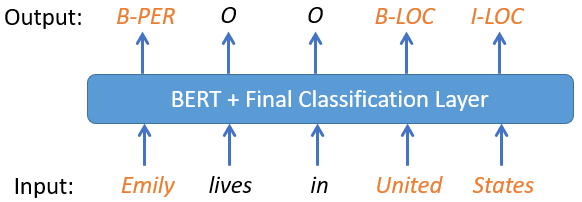
\includegraphics[scale=0.8]{sequence_labeling}
    \caption{Sequence Labeling Setup with \texttt{BIO} tagging scheme (colored tokens are the gold entity mentions and expected output labels)}
    \label{fig:sequence_labeling}
\end{figure}

% \subsection{Experiment Details}
% For \texttt{CNN-LSTM-CRF (BERT-Freeze)} setup, we take the mean of sub-token embeddings from BERT to get the embedding for each input token. We make use of \texttt{BIO} tagging scheme in all our sequence labeling experiments. Models with frozen BERT parameters used learning rate $0.005$. CNN input channels is set to character vocabulary size and each character is fed as a one-hot vector. CNN has $128$ output channels, kernel size of $5$ and does a max pooling to get word-level representation from character-level outputs. LSTM hidden dimensions is set to $256$.

\begin{table}[h!]
\centering
\begin{tabular}{|c|c|c|c|c|}\hline
	\textbf{Model} & \textbf{BioNLP13CG} & \textbf{JNLPBA} & \textbf{CoNLL 2003} & \textbf{OntoNotes 5.0}\\\hline
	\texttt{BERT-Freeze} & 75.42 & 55.93 & 82.79 & 67.35 \\\hline
% 	\texttt{CNN-LSTM-CRF (BERT-Freeze)} & 84.1 & 76.2 & 91.6 & 86.4 \\\hline
	\texttt{BERT} & \textbf{85.99} & \textbf{74.35} & \textbf{91.36} & \textbf{83.39} \\\hline
	\end{tabular}
    \caption{Results: Sequence Labeling (Test set Micro-F1 in \%)}
    \label{tab:res_seq_labeling}
\end{table}

\subsection{Observations}
Based on results summarized in Table \ref{tab:res_seq_labeling} we see that BERT-Freeze serves as a naive yet strong baseline. Nevertheless, as expected, after fine-tuning the BERT model we get much better results since the representative power of the model increases many fold.

% Based on results summarized in Table \ref{tab:res_seq_labeling}:
% \begin{itemize}
%     \item \texttt{BERT-Freeze} serves as a naive yet strong baseline for the other two language models to improve upon.
%     \item Both CNN-LSTM-CRF and transformer-based BERT architecture perform comparably on NER task on these relatively small-sized datasets as can be seen from \texttt{BERT} and \texttt{CNN-LSTM-CRF (BERT-Freeze)} results.
% \end{itemize}

\section{Question Answering}
\label{sec:question_answering}
In recent years there has been a trend of formulating NER problems as question answering(QA) tasks. \cite{li2019entity, levy2017zero} model relation extraction as QA tasks and \cite{mccann2018natural} propose a QA-based multi-task learning setup. 

For NER using a QA setup, we feed a question to the model asking it to extract all mentions of a given entity type from the supplied text. Since there can be multiple entities of interest, each combination of entity question and input sentence is fed to the model. \cite{li2019unified, li2019dice} show the effectiveness of such a setup using BERT over multiple general English and Chinese news datasets and output candidate spans (start and end indices) where the entity in question is present. This setup has advantages over sequence labeling since it can handle nested entities as well. 

However, for learning spans (start and end indices), the classification layer has to do $\mathcal{O}(n^2)$ computations where $n$ is the number of tokens in the input sentence. Such a computation can be expensive for large sentences. To mitigate this, \cite{banerjee2019knowledge} propose an approach in the middle of question answering and sequence labeling. They return \texttt{B}, \texttt{I} and \texttt{O} labels for each token to mark the presence of the entity in question. Hence, their problem complexity becomes $\mathcal{O}(n)$ since they output one label for each token. We implement this framework (shown in Figure \ref{fig:question_answering}) and study the effect of several factors:

\begin{itemize}
    \item \textbf{Tagging Scheme}: Classify each token using \texttt{BIO} or \texttt{BIOE} scheme. In both these models, we ask questions of the form, \textit{What is the person mentioned in the text?}.
    
    \item \textbf{Question Formulation}: In QA setup, extraction from a sentence is highly dependent on the question semantics. We study the importance of the question word being used (\texttt{What} or \texttt{Where}). Our sample question is of the form, \textit{\texttt{What}$\vert$\texttt{Where} is the person mentioned in the text?} In both these models, we follow the \texttt{BIOE} output tagging scheme.
    
    \item \textbf{Entity Scrambling}: In the question, \textit{What is the \texttt{entity} mentioned in the text?}, we study the effect of the entity keyword used. We replace each entity with some scrambled English letters, for example, \texttt{Person} becomes \texttt{xyz12qqr}. So, during training, we ask questions like \textit{What is the \texttt{xyz12qqr} mentioned in the text?} but give the right \texttt{person} mentions as gold labels to the model. Since our task here is to probe the model and develop an understanding of what it focuses on, so we conduct this experiment on a single dataset, \texttt{BioNLP13CG}. Table \ref{tab:entity_scramble_bio} shows some example scrambled entity keywords. We compare it with the unscrambled model in the same \texttt{BIOE} tagging scheme setting.
    
    \begin{table}[h!]
    \centering
    \begin{tabular}{|c|c|}\hline
    	\textbf{Original Entity Name} & \textbf{Scrambled Entity Name}\\\hline
    	\texttt{Cancer} & \texttt{OUYOFhok}\\\hline
    	\texttt{Amino\_acid} & \texttt{DJHkjh KJDSjh}\\\hline
    	\texttt{Organ} & \texttt{UQUIhkjsndf}\\\hline
    	\texttt{Cell} & \texttt{OIFoisjf}\\\hline
    	\end{tabular}
        \caption{Entity Scrambling Examples}
        \label{tab:entity_scramble_bio}
    \end{table}
\end{itemize}

\begin{figure}
    \centering
    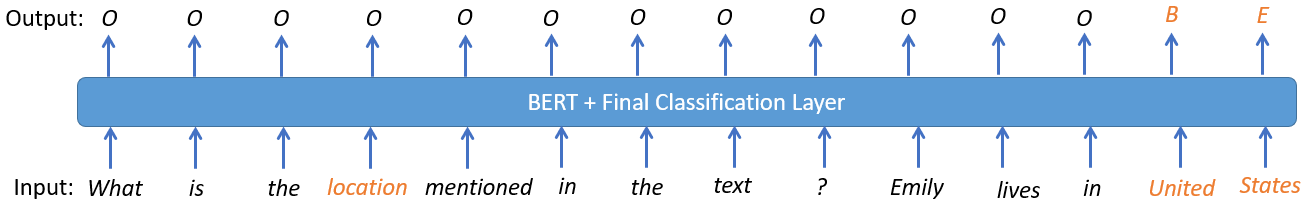
\includegraphics[scale=0.59]{question_answering}
    \caption{Question Answering Setup with \texttt{BIOE} scheme and \textit{What} as question word (colored tokens depict the entity type in question and gold entity mention with expected output labels)}
    \label{fig:question_answering}
\end{figure}

\begin{table}[h!]
\centering
\begin{tabular}{|c|c|c|c|c|}\hline
	\textbf{Model} & \textbf{BioNLP13CG} & \textbf{JNLPBA} & \textbf{CoNLL 2003}\\\hline
	\texttt{BERT-QA(BIO)} & 86.15 & 74.81 & 91.06\\\hline
	\texttt{BERT-QA(BIOE)} & \textbf{86.45} & \textbf{74.92} & \textbf{91.17}\\\hline
	\end{tabular}
    \caption{Results: Question Answering (Tagging Scheme) (Test set Micro-F1 in \%)}
    \label{tab:res_qa_tagging}
\end{table}

\begin{table}[h!]
\centering
\begin{tabular}{|c|c|c|c|}\hline
	\textbf{Model} & \textbf{BioNLP13CG} & \textbf{JNLPBA} & \textbf{CoNLL 2003}\\\hline
	\texttt{BERT-QA(What)} & 86.45 & \textbf{74.81} & 91.17\\\hline
	\texttt{BERT-QA(Where)} & \textbf{86.83} & 74.64 & \textbf{91.82}\\\hline
	\end{tabular}
    \caption{Results: Question Answering (Question Formulation) (Test set Micro-F1 in \%)}
    \label{tab:res_qa_question}
\end{table}

\begin{table}[h!]
\centering
\begin{tabular}{|c|c|}\hline
	\textbf{Model} & \textbf{BioNLP13CG}\\\hline
	\texttt{Original} & \textbf{86.45}\\\hline
	\texttt{Scrambled} & 85.83\\\hline
	\end{tabular}
    \caption{Question Answering (Entity Scrambling) (Test set Micro-F1 in \%)}
    \label{tab:res_qa_scrable}
\end{table}

\subsection{Observations}
\begin{itemize}
    \item From Table \ref{tab:res_qa_tagging}, \texttt{BIOE} tagging is able to better capture the entity boundaries as compared to \texttt{BIO} tagging scheme.
    
    \item From Table \ref{tab:res_qa_question}, we observe that the model is sensitive to slight changes in question semantics. Since the ultimate goal of the model is to identify mention boundaries, asking \texttt{Where} works better than \texttt{What}. 
    
    \item From Table \ref{tab:res_qa_scrable}, we observe that as expected, \texttt{Original} keyword model works better than \texttt{Scrambled}. However the contribution of entity keyword is very minimal. It is possible to form some logical groups of entity mentions with unknown group name and the model should still be able to distinguish and differentiate the group well. We use this finding in Section \ref{sec:clustering}.
\end{itemize}

\section{Span Detection and Classification Pipeline}
\label{sec:span_pipeline}

Previous approaches like sequence labeling and question answering (QA) treat the NER problem as a whole. One single model must take a sentence as input and return mention tuples with correct boundaries and correct entity type. Another possibility is to have a division of labor. We break down the NER problem into a two-step pipelined process. In the first step (\textbf{Span Detector}), we detect all mention spans in a given sentence. In the next step (\textbf{Span Classifier}), we classify these spans into their corresponding entity type. Now, we can train two separate models independently which specialize in their own sub-tasks and together solve the NER problem. We borrow the basic intuitions of QA model to solve both our sub-tasks.

\subsection{Span Detection}
Given a sentence $\mathcal{S}$ as a $N$-length sequence of tokens, $\mathcal{S} = \langle w_1, w_2 \ldots w_N \rangle$, the goal of this module is to output a list of spans (mention tuples) $\langle s, e\rangle$ where $s \in [1, N]$ is the \textit{start} index, $e \in [1, N]$ is the \textit{end} index. Note that here the mention tuples are not associated with an entity type. 

We formulate this as a question answering task asking the model to identify all entity spans in a given sentence. For example, the sentence, \textit{Emily}[\texttt{PERSON}] \textit{lives in United States}[\texttt{LOCATION}], is converted to the input, \textit{What is the \texttt{entity} mentioned in the text? Emily lives in United States}. This is fed to BERT model which outputs labels for each token following the \texttt{BIOE} scheme. In this example, we expect two spans, \textit{Emily} and \textit{United States}. Figure \ref{fig:span_detection} shows our span detection setup.

\begin{figure}
    \centering
    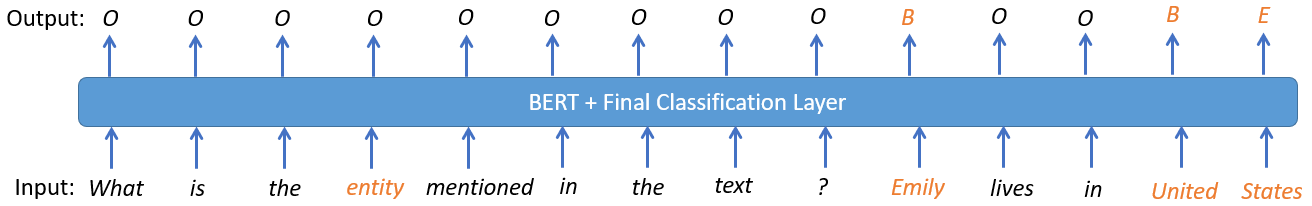
\includegraphics[scale=0.59]{span_detection}
    \caption{Span Detection Setup with \texttt{BIOE} scheme and \textit{What} as question word (colored tokens depict the generic entity type in question and gold entity mentions with expected output labels)}
    \label{fig:span_detection}
\end{figure}

\subsection{Span Classification}
Here, we are given a sentence $\mathcal{S}$ as a $N$-length sequence of tokens, $\mathcal{S} = \langle w_1, w_2 \ldots w_N \rangle$ and a span $\langle s, e\rangle$ where $s \in [1, N]$ is the \textit{start} index, $e \in [1, N]$ is the \textit{end} index. The goal is to output a label $t$ for the span such that $t \in \mathcal{T}$, where $\mathcal{T}$ is the set of all entity types.

This is modeled as the reverse of QA model for NER described in Section \ref{sec:question_answering}. For every gold entity mention (E.g. \textit{United States}) in a training set sentence, \textit{Emily}[\texttt{PERSON}] \textit{lives in United States}[\texttt{LOCATION}], we form a sample input, \textit{Emily lives in United States. What is United States?} The sentence is fed to a BERT model where we do sequence classification. The pooled sequence embedding returned by BERT is fed to a fully connected layer and converted to a probability distribution over possible entity types. In this example, the model is expected to assign maximum probability to \texttt{LOCATION}. Figure \ref{fig:span_classification} shows our span classification setup.

\begin{figure}[h!]
    \centering
    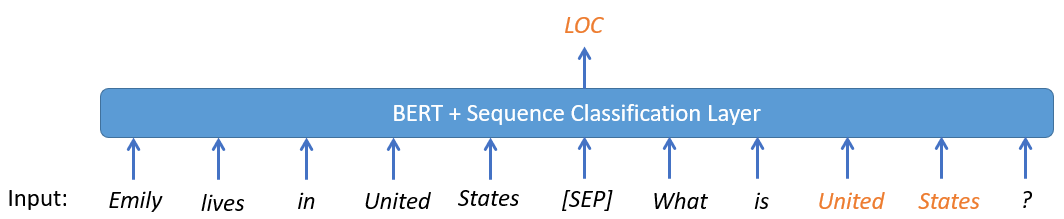
\includegraphics[scale=0.63]{span_classification}
    \caption{Span Classification Setup (colored tokens depict the entity mention in question with expected output entity label)}
    \label{fig:span_classification}
\end{figure}

\subsection{Pipeline}
Both the models can be trained independently. The pipeline structure comes during the inference time. Here, every unlabeled sentence is first passed through Span Detector and for each output span, we convert to an input sample for Span Classifier.

\subsection{Salient Features}

\begin{itemize}
    \item Compared to sequence labeling and question answering approach, this span-based approach has more representative power. This is because here we have two BERT models each working on their own sub-tasks and contributing towards better NER while the other approaches just have a single model.
    
    \item Even though we are training two BERT models, they can be trained independently, in parallel. Only at inference time, we need to maintain the sequential nature.
    
    \item If we have $T$ entities of interest, then standard question answering approach creates $T$ samples for each input sentence both at train and inference time. Considering that each sentence on an average has much lesser than $T$ entity mentions, there is a lot of redundancy in this approach. 
    
    \item Our span-based approach removes QA model redundancy even though inherently we have a QA-based setup. Span Detector only sees an input sentence once and identifies all mention spans. The span classifier will work on only these identified mention spans and classify them into an entity type.
    
    \item Nevertheless, our approach has a pipeline-based structure and hence errors made by span detector propagate to the classifier. Sequence labeling and question answering approaches do not face this concern. 
    
    \item Our span-based approach shows the effectiveness of \textit{reverse question answering}. For a sentence, \textit{Emily lives in United States}, rather than asking a question of the form, \textit{"What is the \texttt{Person} mentioned in the text?"}, we ask, \textit{"What is \texttt{Emily}?"}. This opens up prospects for more intuitive forms of approaching NER, taking us closer to human understanding and interpretations.
    
    \item Comparable and even improved performance of this span-based approach compared to the general QA NER setup (results in Table \ref{tab:res_span}) shows that boundary detection of mentions has less correlation with the entity type it belongs to.
\end{itemize}

\begin{table}[h!]
\centering
\begin{tabular}{|c|c|c|c|c|}\hline
	\textbf{} & \textbf{BioNLP13CG} & \textbf{JNLPBA} & \textbf{CoNLL 2003}\\\hline
	\texttt{Span Detection} & 90.12 & 78.35 & 95.23\\\hline
	\texttt{Span Classification} & 94.06 & 95.08 & 94.50\\\hline
	\texttt{Pipeline} & 85.89 & \textbf{75.01} & \textbf{91.64}\\\hline
	\texttt{BERT-QA} & \textbf{86.45} & 74.81 & 91.17\\\hline
	\end{tabular}
    \caption{Results: Span Pipeline (Test set Micro-F1 in \%)}
    \label{tab:res_span}
\end{table}

\subsection{Observations}
Table \ref{tab:res_span} reports the results of the pipelined span detection and classification procedure and compares it with simple BERT QA setup. We present this comparison since QA model serves as the primary backbone of our span-based approach. All models here use \texttt{BIOE} tagging scheme and use \textit{What} as the question word in question formulation.

\begin{itemize}
    \item \textbf{Span Detection}: Detecting all mention spans together without classification is a simpler problem for the model than full NER and we get better performance on this sub-task compared to complete NER task in QA setup.
    
    \item \textbf{Span Classification}: Given that spans are pre-identified, classifying them to an entity type is a relatively simple task for the BERT model. On all datasets, we see around $95\%$ Micro-F1 on test set.
    
    \item \textbf{Pipeline}: The pipelined procedure gives comparable and even better performance than standard QA NER model on all datasets demonstrating the effectiveness of this division of labor. 
    
    \item Since out \texttt{Pipeline} results are comparable to \texttt{BERT-QA} model, we conclude that internally \texttt{BERT-QA} model also tries to logically segregate boundary detection and classification as separate tasks.
    
    \item The results of span pipeline are limited by the performance of the span detector part. Since this procedure is pipelined, errors in this first step propagate to the next step. Boundary detection serves as the primary challenge in Span Detector and has a large scope for improvement on biomedical datasets.
    
    \item Qualitative analysis reveals that both \texttt{BERT-QA} and \texttt{Span Detector} share very similar boundary detection issues as highlighted in Section \ref{subsec:qualitative_analysis}.
\end{itemize}

\section{Learning Objective Variation}
An ML algorithm learns by optimizing its learning objective (loss function). In this section, we use some standard popular loss functions and also design our new ones and study their effect on model performance. In all our experiments here, we use sequence labeling setup with \texttt{BIO} tagging scheme. Without loss of generality, we use the binary classification setting while illustrating the different loss functions. Let $\mathcal{X}$ be the set of all training samples such that a sample $x_i \in \mathcal{X}$ is associated with ground truth label, $y_i = [y_{i0}, y_{i1}]$ where $y_{i0}, y_{i1} \in \{0, 1\}$. Let $p_i = [p_{i0}, p_{i1}]$ be model prediction probabilities such that $p_{i0}, p_{i1} \in [0, 1]$ and $p_{i0} + p_{i1} = 1$. Let $N$ be the batch size.

\subsection{Cross Entropy (CE) Loss}
As can be seen from Equation \eqref{eq:cross_entropy}, Cross Entropy loss penalizes misclassifications. When the classification is correct, it pushes the model to output the correct result with a probability of 1. Hence, Cross Entropy loss models accuracy. However, during evaluation in NER setting, we calculate F1-Score. This difference between training objective and evaluation metric may lead to sub-optimal performance in some situations.
\begin{equation}
\label{eq:cross_entropy}
    CE = -\frac{1}{N}\sum_{i}\sum_{j \in \{0, 1\}} y_{ij}\log p_{ij}
\end{equation}

\subsection{Weighted CE Loss}
Not all entity types may have an equable distribution in the labeled dataset. Generally negative samples outweigh positive samples in NER datasets. Only $23.5\%$ tokens in \texttt{BioNLP13CG} dataset belong to some entity, rest are labeled \texttt{O}. This may introduce bias in the model which can be countered by giving different importance/weights to different entity types. In our case, we want to reduce the dominant influence of \texttt{O} labels, hence, any token with a gold label \texttt{O} is given a weight of $0.5$ while all others have a weight of $1$. This can be further extended to give different weights to high and low resource entity types. However, this approach makes the model very sensitive to the assigned weights and it can rather easily develop a bias towards low-resource entities\cite{valverde2017improving}.

\subsection{Punctuation Weighted CE Loss}
From qualitative analysis of misclassified samples (Section \ref{subsec:qualitative_analysis}) in standard CE loss setup we notice that the model is not able to learn good representations for special symbols like parenthesis, hyphen, period, or slash. Hence, we emphasize these symbols by penalizing the model twice if the misclassified token is a punctuation/special symbol.

\subsection{Dice Loss}
As detailed earlier, Cross Entropy is an accuracy-oriented objective while during evaluation, we calculate the F1-Score. This difference can lead to sub-optimal model training. To counteract, \cite{li2019dice} make use of S{\o}rensen-Dice coefficient(DSC)\cite{sorensen1948method, dice1945measures} and Tversky index\cite{tversky1977features} which are F-Score oriented statistics. Given sets $A$ and $B$, DSC is used to gauge similarity among two sets and is defined as,
\begin{equation}
\label{eq:dsc_set}
    DSC(A, B) = \frac{2\ \vert A \cap B \vert}{\vert A \vert + \vert B \vert}
\end{equation}
Consider $A$ as set of all positive samples predicted by a model and $B$ as set of all ground truth positives. Then, by definition of true positive ($TP$), false positive ($FP$) and false negative ($FN$) from Section \ref{sec:evaluation_metrics}, we have,
\begin{equation}
\label{eq:dsc_tp}
    TP = \vert A \cap B \vert
\end{equation}
\begin{equation}
\label{eq:dsc_a}
    \vert A \vert = TP + FP
\end{equation}'
\begin{equation}
\label{eq:dsc_b}
    \vert B \vert = TP + FN
\end{equation}
Using Equations \ref{eq:dsc_tp}, \ref{eq:dsc_a} and \ref{eq:dsc_b}, in Equation \ref{eq:dsc_set}, we get,
\begin{equation}
\label{eq:dsc_as_f1}
     DSC(A, B) = \frac{2TP}{2TP + FP + FN} = \frac{2\ \frac{TP}{TP + FN}\ \frac{TP}{TP + FP}}{\frac{TP}{TP + FN} + \frac{TP}{TP + FP}} = \frac{2\ Precision \times Recall}{Precision + Recall} = F1
\end{equation}

The dice coefficient gives equal importance to false-positives and false-negatives at training time and is more immune to data-imbalance issues\cite{sudre2017generalised, shen2018influence, kodym2018segmentation}. The above formulation (Equation \ref{eq:dsc_as_f1}) shows its equivalence to F1-score thus removing the discrepancy among training and evaluation metrics. From Equation \ref{eq:dsc_set}, for an individual sample $x_i$, dice coefficient is defined as,
\begin{equation}
\label{eq:dsc_per_sample}
    DSC(x_i) = \frac{2p_{i1}y_{i1} + \gamma}{p_{i1} + y_{i1} + \gamma}
\end{equation}
where $\gamma$ is the smoothing parameter. Then over all samples, from Equation \ref{eq:dsc_per_sample}, dice loss (DL) is defined in Equation \ref{eq:dice_loss} as:
\begin{equation}
\label{eq:dice_loss}
    DL = 1 - \frac{2\sum_i{p_{i1}y_{i1}} + \gamma}{\sum_i{p_{i1}} + \sum_i{y_{i1}} + \gamma}
\end{equation}

\subsection{Conditional Random Field}
\cite{ma2016end} show the effectiveness of a conditional random field (CRF) in modeling output label transitions in sequence labeling settings when added over a bidirectional LSTM. In this setup, we apply a similar CRF layer on top of BERT for assigning output labels to each token. For CRF implementation, we use \texttt{torchcrf} python package.

\begin{table}[h!]
\centering
\begin{tabular}{|c|c|c|c|c|}\hline
	\textbf{} & \textbf{BioNLP13CG} & \textbf{CoNLL 2003}\\\hline
	\texttt{CE Loss} & 85.99 & 91.36\\\hline
	\texttt{Weighted CE Loss} & 85.93 & 91.26\\\hline
	\texttt{Punctuation CE Loss} & 85.74 & 91.55\\\hline
	\texttt{Dice Loss} & 86.35 & 90.76\\\hline
	\texttt{CRF} & 86.20 & 91.23\\\hline
	\end{tabular}
    \caption{Results: Learning Objectives (Test set Micro-F1 in \%)}
    \label{tab:res_loss}
\end{table}

\subsection{Observations}
\begin{itemize}
    \item \texttt{Weighted CE Loss} and \texttt{Punctuation CE Loss} give mixed results. Their performance varies with the weights set for different misclassification cases. The same set of weights do not generalize across both datasets.
    
    \item In \texttt{BioNLP13CG} corpus, \texttt{Dice Loss} performs well as this corpus as several high and low resource entities (data imbalance). \texttt{Dice Loss} is not able to give its advantages with \texttt{CoNLL 2003} corpus since here all 4 entity types have a comparable and high representation.
    
    \item From a sequence labeling perspective with \texttt{BIO} tagging scheme, we get $2K + 1$ output entity classes for $K$ entity types. This means \texttt{BioNLP13CG} corpus with $16$ entity types requires $33$ output classes and \texttt{CoNLL 2003} with $4$ entities requires $9$ output classes. A \texttt{CRF} primarily captures tag transitions and is found to be helpful when number of output labels is more, that is, on \texttt{BioNLP13CG} corpus. On \texttt{CoNLL 2003} data, it gives comparable performance to the base model.
\end{itemize}

\section{Capturing Additional Token Semantics}
\label{sec:additional_token_semantics}
After having run through the three major approaches for NER namely, sequence labeling, question answering and span detection and classification, in this section we present a qualitative error analysis. Next, we address the identified issues by either architectural modification or additional input features.

\subsection{Qualitative Error Analysis}
\label{subsec:qualitative_analysis}

Different approaches have their own strengths and weaknesses highlighted later in Section \ref{sec:precision_recall_analysis}. However there are several common errors which can be segregated into three major categories:

\begin{itemize}
    \item \textbf{Out of Vocabulary Terms}: Both in news articles and research texts, it is common to coin new terms and abbreviations to describe latest events or new concepts. Such terms are pretty much localized to that article and rare otherwise. Additionally scientific texts also have chemical formulas which have numerals encoded within. Semantics of many such terms may not be captured well by generically pretrained BERT models. Although BERT uses sub-word semantics using WordPiece tokenizer but such sub-word combinations may still be rare. Hence we call these \textit{out-of-vocabulary} terms. Table \ref{tab:oov_issue} shows some errors made by our models on \texttt{BioNLP13CG} corpus which fall in this category.
    
    \begin{table}[h!]
    \centering
    \begin{tabular}{|c|c|}\hline
    	\textbf{Entity} & \textbf{Misclassification Examples}\\\hline
    	\texttt{Gene\_or\_Gene\_Product} & DPD, Xhol, mutCK1delta, FAS\\\hline
    	\texttt{Simple\_Chemical} & MnCl2, AglRhz, NO\\\hline
    	\texttt{Cell} & LoVo, DeltaG45, BMSVTs\\\hline
    	\texttt{Amino\_Acid} & phosphoS727, Y705F\\\hline
    	\end{tabular}
        \caption{Out-of-Vocabulary terms in \texttt{BioNLP13CG} corpus}
        \label{tab:oov_issue}
    \end{table}
    
    \item \textbf{Special Symbols}: Several entity mentions have hyphens, periods, parenthesis within them. Pretrained embeddings do not capture their semantics well leading to boundary detection issues. Table \ref{tab:boundary_issue} shows some errors of this type from \texttt{BioNLP13CG} dataset.
    
    \item \textbf{Modifier Suffix/Prefix}: Apart from the root entity required to be extracted the gold labels sometimes expect a modifier term as well which occurs as a prefix/suffix. Missing these leads to boundary detection issues. Table \ref{tab:boundary_issue} lists some error cases of this type from \texttt{BioNLP13CG} corpus.
    
    \begin{table}[h!]
    \centering
    \begin{tabular}{|c|c|c|}\hline
    	\textbf{Misclassification Category} & \textbf{Gold} & \textbf{Predicted}\\\hline
    	\texttt{Special Symbols} & L . Se ( + ) cells & L . Se\\\hline
    	\texttt{Special Symbols} & Gs - IB ( 4 - ) ion & Gs - IB ( 4\\\hline
    	\texttt{Modifier Suffix/Prefix} & epicardial coronary artery & coronary artery\\\hline
    	\texttt{Modifier Suffix/Prefix} & T140 analogs & T140\\\hline
    	\end{tabular}
        \caption{Boundary detection issues in \texttt{BioNLP13CG} corpus}
        \label{tab:boundary_issue}
    \end{table}
\end{itemize}

In general, we conclude that for a gold entity mention $\langle s, e, t \rangle$ where $s$ and $e$ represent the span boundaries and $t$ represents entity type, the detection of accurate boundary indices ($s$ and $e$) serves as a primary bottleneck of all current NER approaches discussed. Given a correct mention span, classifying it into an entity type $t$ is relatively simpler, as observed in Section \ref{sec:span_pipeline}.

\subsection{Experiment Details}

To address the above mentioned issues, we provide additional inputs and infrastructure to the model to learn the underlying semantics better. In these experiments, we develop on top of the sequence labeling setup with \texttt{BIO} tagging scheme.

\begin{itemize}
    \item \textbf{Special Symbol Features}: Before feeding to final classifier, concatenate BERT hidden layer output with a one-dimensional vector, set if the input token is a pure special symbol. This means we assign $1$ for \textit{hyphen}(\texttt{-}), \textit{parenthesis}(\texttt{(} and \texttt{)}), and \textit{comma}(\texttt{,}). Terms like \texttt{carbon}, \texttt{123}, \texttt{Ca(2+)}, and \texttt{AB-3} get assigned $0$.
    
    \item \textbf{Word Type Features}: As an extension to special symbol features, here we associate each input token with a word type (shown in Table \ref{tab:word_type_encoding}) which is converted into a one-hot vector concatenated with BERT output embeddings before feeding to the classifier layer.
    
    \begin{table}[h!]
    \centering
    \begin{tabular}{|c|c|}\hline
    	\textbf{Word Type} & \textbf{Encoding}\\\hline
    	\texttt{[CLS] token} & 0\\\hline
    	\texttt{[SEP] token} & 1\\\hline
    	\texttt{all lowercase} & 2\\\hline
    	\texttt{all caps} & 3\\\hline
    	\texttt{first letter caps, rest lowercase} & 4\\\hline
    	\texttt{all digits} & 5\\\hline
    	\texttt{all special symbols} & 6\\\hline
    	\texttt{alphabets + digits} & 7\\\hline
    	\texttt{all the rest} & 8\\\hline
    	\end{tabular}
        \caption{Word Type Encoding}
        \label{tab:word_type_encoding}
    \end{table}
    
    \item \textbf{Character and Pattern Features}: Chemical formulas and scientific terms generally follow a nomenclature convention or pattern. Similarly, out-of-vocabulary terms may have some intrinsic character-level information which is not well captured by the sub-words fed to the BERT model. \cite{boukkouri2020characterbert} study this issue and propose a character-CNN instead of WordPiece tokenizer at the input stage to the BERT model. Motivated by the CNN-LSTM-CRF\cite{ma2016end} model and this study, we do the following:
    
    \textbf{Modeling characters}. Each word is passed to BERT and simultaneously to five one-dimensional CNNs with kernel sizes of $1$ to $5$, each having $16$ input and $16$ output channels. Input character is indexed and mapped to a $16$-dimensional embedding. Character-level outputs are max-pooled to get word representation. Outputs from multiple CNNs are concatenated and passed through a linear layer to get overall $768$-dimensional output vector for each token.
    
    \textbf{Modeling patterns}. Each word is converted to a pattern (a regular expression or a denser space with smaller character set). For example, all uppercase letters are mapped to \texttt{U}, lowercase to \texttt{L}, and digits to \texttt{D}. These patterns are then fed to a Character-CNN (like the one described above) and then to a bidirectional LSTM to get contextual pattern token embeddings.
    
    Finally, these character and pattern embeddings are concatenated with BERT outputs and fed to final classifier layer.
    
    \item \textbf{Part-of-Speech and Dependency Parse Features}: Concatenate BERT embeddings with the one-hot part-of-speech and dependency parse features before feeding to final classifier layer. The part-of-speech and dependency parse tags are generated using \texttt{scispacy} for \texttt{BioNLP13CG} and \texttt{JNLPBA} datasets, \texttt{spacy} for \texttt{CoNLL 2003} and \texttt{OntoNotes 5.0} datasets.
    
    \item \textbf{Head Tokens}: BERT uses WordPiece tokenizer and may break a single input token into multiple sub-words. Instead of doing token classification on each of these sub-words and making sure everything is correct, it is simpler to take the BERT hidden layer output for the first (\textit{head}) sub-word for each token. This technique is also used in the original BERT paper\cite{devlin2018bert} for NER.
    
    \item \textbf{Highway Network}: Instead of directly concatenating character-based features with BERT, we create a highway network\cite{srivastava2015highway} similar to the one used in BiDAF\cite{seo2016bidirectional} architecture and train a logic gate to control the inflow of information from BERT vectors and additional character-level semantics.
\end{itemize}

\begin{table}[h!]
\centering
\begin{tabular}{|c|c|c|}\hline
	\textbf{Model} & \textbf{BioNLP13CG} & \textbf{CoNLL 2003}\\\hline
	\texttt{Vanilla BERT} & 85.99 & 91.36\\\hline
	\texttt{Special Symbol} & 86.63 & 91.67\\\hline
	\texttt{Word Type} & 86.50 & 91.55\\\hline
	\texttt{Character/Patterns} & 86.44 & 91.08\\\hline
	\texttt{Part-Of-Speech} & 86.11 & 91.47\\\hline
	\texttt{Dependency Parse} & 86.20 & 91.32\\\hline
	\texttt{Head Tokens} & 86.17 & 91.49\\\hline
	\texttt{Special Symbol + Head Tokens} & 86.36 & 91.68\\\hline
	\texttt{Highway Net} & 85.77 & 91.53\\\hline
	\end{tabular}
    \caption{Results: Token Semantics (Test set Micro-F1 in \%)}
    \label{tab:res_token_semantics}
\end{table}

\subsection{Observations}
Our results are summarized in Table \ref{tab:res_token_semantics}. We also experimented with combinations of the above described features together but omit the results from this report if not found to be significant. We make the following observations:

\begin{itemize}
    \item Almost all of the proposed additional features are found to improve upon the \texttt{Vanilla BERT} model on both \texttt{BioNLP13CG} and \texttt{CoNLL 2003} datasets.
    
    \item Handling special symbols is a primary issue of \texttt{Vanilla BERT}. Explicitly handling it is found to be most helpful among all the other features across both datasets and on both models \texttt{Special Symbol} and \texttt{Special Symbol + Head Tokens}.
    
    \item Extending the special symbol features to word types gives mixed signals to the model. \texttt{Word Type} model hence gives the second best performance on both datasets.
    
    \item \texttt{Character/Patterns} modeling helps in the biomedical text setting since it helps understand semantics of chemical names. However, giving importance to intrinsic patterns gives conflicting signals for general English entities and hence gives lower performance on \texttt{CoNLL 2003} data.
    
    \item \texttt{Part-of-Speech} and \texttt{Dependency Parse} features give some additional insights to the model over \texttt{Vanilla BERT} and hence give comparable or even better performance. 
    
    \item Considering only \texttt{Head Tokens} helps over \texttt{Vanilla BERT} on both datasets. \texttt{Special Symbol + Head Tokens} gives the best performance on \texttt{CoNLL 2003} data. The improvement is reduced compared to \texttt{Special Symbol} on the \texttt{BioNLP13CG} data. We suspect this is because of the loss of intrinsic sub-word details which can be crucial for biomedical text since they have lots of out-of-vocabulary chemical/gene names.
    
    \item \texttt{Highway Net} rightly ignores confusing character-level information for \texttt{CoNLL 2003} data and hence gives a performance boost over \texttt{Character/Patterns}. For the \texttt{BioNLP13CG} data, this additional highway layer is unable to give improvements since it adds undesired complexity to the model.
\end{itemize}

\section{Training Effectiveness Study}
In section \ref{sec:additional_token_semantics}, we looked at some limitations of the pretrained BERT model in capturing special symbols and rare word semantics. To counteract, we proposed feeding in some additional token semantics. In this section, we study how effectively the model is able to pick cues and learn from the supplied additional features. Our experiments are conducted in sequence labeling setting on \texttt{BioNLP13CG} corpus using \texttt{BIO} tagging scheme.

\subsection{Feeding Answer as Input}
To study the training effectiveness, we give the model the best ideal-case information, that is, for each token, we feed its gold label as a one-hot vector. This is concatenated with BERT outputs before feeding to final classifier. We study the following variants:

\begin{itemize}
    \item \texttt{BERT(Freeze) + Answer}: We concatenate BERT outputs with answer vectors and freeze BERT model parameters during training. This effectively reduces the no. of trainable parameters to around $26,000$. We train this in two settings, low learning rate of $10^{-5}$ (recommended BioBERT learning rate\footnote{https://github.com/dmis-lab/biobert\#named-entity-recognition-ner}) and high learning rate of $0.005$.
    
    \item \texttt{BERT + Answer}: This mimics the standard setting where the BERT model is fine-tuned with given additional information at a low learning rate of $10^{-5}$.
    
    \item For comparison with the above variants, we also present the results for simple \texttt{BERT} (fine-tuned) and \texttt{BERT(Freeze)} models as well (without any answer inputs).
\end{itemize}

\begin{table}[h!]
\centering
\begin{tabular}{|c|c|c|}\hline
	\textbf{Model} & \textbf{Learning Rate} & \textbf{BioNLP13CG}\\\hline
	\texttt{BERT} & $10^{-5}$ & $85.99$\\\hline
	\texttt{BERT + Answer} & $10^{-5}$ & $86.35$\\\hline
	\texttt{BERT(Freeze)} & $0.005$ & $75.42$\\\hline
	\texttt{BERT(Freeze) + Answer} & $0.005$ & $100.00$\\\hline
	\texttt{BERT(Freeze) + Answer} & $10^{-5}$ & $63.89$\\\hline
	\end{tabular}
    \caption{Results: Training Effectiveness - Feed Answer as Input (Test set Micro-F1 in \%)}
    \label{tab:res_training_ans_input}
\end{table}

From results summarized in Table \ref{tab:res_training_ans_input}, we make the following observations:
\begin{itemize}
    \item From \texttt{BERT} and \texttt{BERT(Freeze)}, we conclude that fine-tuning the model definitely helps.
    
    \item From \texttt{BERT} and \texttt{BERT + Answer}, we observe that feeding the answer with input gives better performance. However at a low learning rate of $10^{-5}$, the gain is very small.
    
    \item From \texttt{BERT(Freeze) + Answer} at learning rates $0.005$ and $10^{-5}$, we observe that at low learning rate the model is not able to effectively catch the provided cues. At high learning rate, we get perfect scores as expected.
\end{itemize}

\subsection{What happens at high learning rate?}
From the previous section, we see that model needs training at high learning rate for learning from additional input features. But with BERT fine-tuning, it is recommended\footnote{https://github.com/dmis-lab/biobert\#named-entity-recognition-ner} to use a low learning rate in the order of $10^{-5}$. To study this, we pass gold mention spans as input to the model. Basically, for each token we add a one-dimensional vector which is set if the token is a part of some gold entity mention. This means effective the model just has to do span classification which is a relatively easy task as seen previously in Section \ref{sec:span_pipeline}. We experiment with the following variants:

\begin{itemize}
    \item \texttt{BERT(Freeze) + Gold Span}: Concatenate last hidden layer output from BERT with gold-labeled span vectors. and freeze BERT parameters during training. This model is expected to perform better than \texttt{BERT(Freeze)}.
    
    \item \texttt{BERT + Gold Span}: Same as the above model but with BERT fine-tuning. We train this in two settings, with low learning rate of $10^{-5}$ and high learning rate of $0.005$.
    
    \item We also present \texttt{BERT} (fine-tuned) and \texttt{BERT(Freeze)} results for comparison.
\end{itemize}

\begin{table}[h!]
\centering
\begin{tabular}{|c|c|c|}\hline
	\textbf{Model} & \textbf{Learning Rate} & \textbf{BioNLP13CG}\\\hline
	\texttt{BERT(Freeze)} & $0.005$ & $75.42$\\\hline
	\texttt{BERT(Freeze) + Gold Span} & $0.005$ & $79.18$\\\hline
	\texttt{BERT} & $10^{-5}$ & 85.99\\\hline
	\texttt{BERT + Gold Span} & $10^{-5}$ & $85.78$\\\hline
	\texttt{BERT + Gold Span} & $0.005$ & $0.0$\\\hline
	\end{tabular}
    \caption{Results: Training Effectiveness - Feed Gold Span as Input (Test set Micro-F1 in \%)}
    \label{tab:res_training_span_input}
\end{table}

From Table \ref{tab:res_training_span_input}, we make the following observations:

\begin{itemize}
    \item From \texttt{BERT(Freeze)} and \texttt{BERT(Freeze) + Gold Span}, we observe that indeed giving gold span information helps the model.
    
    % \item From \texttt{BERT(Freeze) + Gold Span} and \texttt{BERT + Gold Span (LR: $10^{-5}$)}, we observe that indeed fine-tuning is able to learn the semantics of entities much better than when using the BERT embeddings right out-of-the-box.
    
    \item From \texttt{BERT} and \texttt{BERT + Gold Span} at learning rate $10^{-5}$, we observe that with a low learning rate, the model is not able to focus on and effectively utilize the gold span information (similar to our previous findings with answer inputs).
    
    \item From \texttt{BERT + Gold Span} at learning rates $10^{-5}$ and $0.005$, we observe that increasing the learning rate has a deteriorating effect on the pretrained BERT parameters and the rigorous push from a high learning rate pushes the model to an unsatisfactory local optima.
\end{itemize}

% \section{Tagging Scheme Variation}
% As described in Section \ref{sec:tagging_scheme}, in this section, we study how much impact do different output tagging schemes have on boundary detection and learning of the model. We test the \texttt{2-Tag}, \texttt{BIO} and \texttt{BIOE} tagging schemes in question answering setup on \texttt{BioNLP13CG} corpus.

% We omit the experiments with sequence labeling setup since for \texttt{K} output tags, \texttt{2-Tag} scheme gives \texttt{K + 1} output tags (\texttt{+1} for \texttt{O} tag). With \texttt{BIO} scheme, we have \texttt{2K + 1} output tags and with \texttt{BIOE} scheme, we have \texttt{3K + 1} tags. For \texttt{BioNLP13CG} corpus which already has \texttt{K = 16}, the \texttt{BIOE} scheme makes number of output tags as \texttt{49}, which is too large to train well since we don't have enough training data. However, for the question answering setup, the number of output tags remains \texttt{3} for \texttt{2-Tag}, \texttt{4} for \texttt{BIO} and \texttt{5} for \texttt{BIOE} scheme which is manageable.

% \begin{table}[h!]
% \centering
% \begin{tabular}{|c|c|}\hline
% 	\textbf{Model} & \textbf{BioNLP13CG}\\\hline
% 	\texttt{BERT-QA (2-Tag)} & todo\\\hline
% 	\texttt{BERT-QA (BIO)} & 86.15\\\hline
% 	\texttt{BERT-QA (BIOE)} & 86.45\\\hline
% 	\end{tabular}
%     \caption{Results: Tagging Scheme Variation in QA Setup (Test set Micro-F1 in \%)}
%     \label{tab:res_tagging_scheme_qa}
% \end{table}

% From results in Table \ref{tab:res_tagging_scheme_qa}, we observe that as expected, explicitly modeling the begin and end boundaries performs the best while not modeling start and end at all, in \texttt{2-Tag} scheme performs the least among them. However this will have lesser number of parameters to train and more representative samples for each case.

\section{Pretrained Model Variation}
In all the experiments done in this work, pretrained BERT model serves as our model backbone. However based on which dataset the pretrained model is trained on and what learning objective is used, there are several variants. We study the effect of this pretraining procedure on NER performance in sequence tagging setup through the following variants: 

\begin{itemize}
    \item \texttt{BERT-Base-Uncased}: Proposed by \cite{devlin2018bert}, this model is trained on English text from Wikipedia and BookCorpus\cite{moviebook} which totals around 16GB of uncompressed text. The model is uncased. It is trained on masked language modeling (MLM) and next sentence prediction objective. We use \texttt{bert-base-uncased} model provided by HuggingFace\footnote{https://huggingface.co/bert-base-uncased} for our \texttt{CoNLL 2003} and \texttt{OntoNotes 5.0} corpora.
    
    \item \texttt{RoBERTa-Base}: Proposed by \cite{liu2019roberta}, this model is trained on English text from 5 different datasets totalling around 160 GB of uncompressed text. The model is cased and trained on only the masked language modeling (MLM) objective. We use \texttt{roberta-base} model provided by HuggingFace\footnote{https://huggingface.co/roberta-base} for our \texttt{CoNLL 2003} and \texttt{OntoNotes 5.0} corpora.
    
    \item \texttt{BioBERT-Base}: Proposed by \cite{lee2020biobert}, this model is trained on English biomedical literature including PubMed abstracts and PMC full text articles. The model is cased and trained on same MLM and next sentence prediction objectives proposed in standard BERT model. We use \texttt{BioBERT-Base v1.1} model provided on GitHub\footnote{https://github.com/dmis-lab/biobert\#download} and import it in HuggingFace as \texttt{dmis-lab/biobert-base-cased-v1.1}. We use this for \texttt{BioNLP13CG} and \texttt{JNLPBA} datasets, since models pretrained on biomedical and scientific texts are found to capture similar semantics more effectively than those trained on general English text.
    
    \item \texttt{SciBERT-Base-Uncased}: Proposed by \cite{beltagy2019scibert}, this model is trained on full texts of papers on Semantic Scholar\footnote{https://www.semanticscholar.org/}. The model is uncased and trained using the MLM and next sentence prediction objectives originally proposed by the BERT paper. However, this model uses \texttt{SciVocab}, a specially created WordPiece vocabulary for scientific texts. Just like BioBERT, we use this for \texttt{BioNLP13CG} and \texttt{JNLPBA} datasets.
    
\end{itemize}

\begin{table}[h!]
\centering
\begin{tabular}{|c|c|c|}\hline
	\textbf{Model} & \textbf{BioNLP13CG} & \textbf{JNLPBA}\\\hline
	\texttt{BERT-Base-Uncased} & $82.63$ & $73.03$\\\hline
	\texttt{BioBERT-Base} & $85.99$ & $74.35$\\\hline
	\texttt{SciBERT-Base-Uncased} & $86.01$ & $74.68$\\\hline
	\end{tabular}
    \caption{Results: Pretrained (Biomedical) Model Variation (Test set Micro-F1 in \%)}
    \label{tab:res_pretrained_model_bio}
\end{table}

\begin{table}[h!]
\centering
\begin{tabular}{|c|c|c|}\hline
	\textbf{Model} & \textbf{CoNLL 2003} & \textbf{OntoNotes 5.0}\\\hline
	\texttt{BERT-Base-Uncased} & $91.36$ & $83.39$\\\hline
	\texttt{RoBERTa-Base} & $91.19$ & $86.34$\\\hline
	\end{tabular}
    \caption{Results: Pretrained (General) Model Variation (Test set Micro-F1 in \%)}
    \label{tab:res_pretrained_model_general}
\end{table}

In Tables \ref{tab:res_pretrained_model_bio} and \ref{tab:res_pretrained_model_general}, we present our results. We observe that:

\begin{itemize}
    \item On \texttt{OntoNotes 5.0} data, \texttt{RoBERTa-Base} performs better than \texttt{Bert-Base-Uncased}. This gives us an insight that case of tokens plays an important role in general English news data. However, on \texttt{CoNLL 2003}, the performance is similar. On investigating further\footnote{https://github.com/google-research/bert/issues/223\#issuecomment-649619302}, we identify that original \texttt{CoNLL 2003} data has some casing issues which people try to resolve by doing truecasing as a pre-processing step. It is because of this casing issue that \texttt{RoBERTa-Base} model is not able to show its advantages on \texttt{CoNLL 2003} data.
    
    \item \texttt{SciBERT-Base-Uncased} performs marginally better than \texttt{BioBERT-Base v1.1} on both biomedical datasets. As expected, both of these domain-specific pretrained models perform much better than \texttt{BERT-Base-Uncased}. 
\end{itemize}

\section{Partitioning Diverse Entities}
\label{sec:clustering}
From the entity distribution in \texttt{BioNLP13CG} dataset (Table \ref{tab:bio_entity_distribution}), we see that entities like \texttt{Cancer} and \texttt{Gene\_or\_gene\_product} are high-resource entity types. They may have high mention diversity and hence it may be difficult for a model to capture all their mention representations. Instead, it may be easier to break a heterogeneous entity class into relatively homogeneous sub-entity classes and work with them. At inference time, remap the sub-entities to the original entity and report F1-scores.

\subsection{Experiment Details}
We work with \texttt{BioNLP13CG} dataset using question answering setup on only 3 entities, \texttt{Gene\_or\_gene\_product}, \texttt{Cancer} and \texttt{Simple\_chemical}. All other entities are ignored. We partition \texttt{Gene\_or\_gene\_product} (the largest entity class) into $K$ sub-entities ($K$ becomes a hyper-parameter). The procedure is described below:

\begin{itemize}
    \item Collect all mentions of \texttt{Gene\_of\_gene\_product}. Pass their corresponding sentences to pretrained \texttt{BioBERT-Base-Uncased} model. Calculate contextualized mention embedding as the concatenation of BERT outputs of first and last sub-words of the mention.
    
    \item For multiple instances of same mention, take the mean of contextual mention embeddings across sentences.
    
    \item Reduce mention embeddings to 100-dimensional vectors using principal component analysis (PCA). Then take their tSNE\cite{van2008visualizing} projections to convert each mention to a 2-dimensional vector representation.
    
    \item \textbf{Clustering}: Fix $K = 4$ (number of clusters). Randomly select $K$ mention instances as cluster centers and apply K-Medoids clustering. Use euclidean distance among tSNE projections as the distance metric\footnote{We evaluated cosine distance and KL-Divergence on tSNE and PCA vectors as distance metrics as well. However the presented setup is found to work the best.}.
    
    \item After clustering, we relabel the corpus tagging each mention to its cluster. Each cluster is considered a sub-entity of \texttt{Gene\_of\_gene\_product}. The sub-entities are named from \texttt{Gene\_of\_gene\_product0} to \texttt{Gene\_of\_gene\_product3}.
    
    \item Next we train a question answering NER model with this new labeled dataset. Note that in Section \ref{sec:question_answering} we saw that the keyword used to represent an entity does not play a crucial role in extraction performance. So, our sub-entity naming convention should not be a problem.
    
    \item During inference time, the model mention with their sub-entity types. We post-process the labels and map each sub-entity output to \texttt{Gene\_of\_gene\_product} and then calculate overall Micro-F1.
\end{itemize}

\begin{table}[h!]
\centering
\begin{tabular}{|c|c|}\hline
	\textbf{Model} & \textbf{BioNLP13CG}\\\hline
	\texttt{BERT-QA} & 87.97\\\hline
	\texttt{BERT-QA (With Partitioning)} & 86.66\\\hline
	\end{tabular}
    \caption{Results: Partitioning Diverse Entities (Test set Micro-F1 in \% on 3 high-resource entities)}
    \label{tab:res_clustering}
\end{table}

\subsection{Observations}
From results in Table \ref{tab:res_clustering}, we observe that entity partitioning technique gives slightly reduced performance compared to original setup. This is because our current clustering is on the basis of semantic similarity captured by BERT embeddings and not similarity among word patterns. As an example, among \texttt{Simple\_chemical}, we want formulas like \textit{CaSO4} to be segregated from names like \textit{calcium sulphate}. However, the BERT model clubs them into the same sub-entity since they are semantically same. Hence, our sub-entities still have high heterogeneity and not well separated, making it difficult for the model to train well. However, with better word-pattern oriented clusters, this technique has potential to give better results.

% \section{Handling Nested Entities}

% As described in \ref{sec:nature_of_entities}, not always are entities of interest completely disjoint of each other in a sentence. There may be nested and overlapping cases. Such examples are frequent in biomedical and news-based datasets like GENIA\cite{kim2003genia}, ACE-2004\cite{mitchell2005ace} and ACE-2005\cite{walker2006ace}. As reported by \cite{finkel2009nested}, around $17\%$ of named entities in GENIA are nested. In biomedical texts, it is common to find nested \texttt{Chemical} and \texttt{Gene} instances, for example, \textit{tyrosine} is a \texttt{Chemical} while \textit{tyrosine kinase} is a \texttt{Gene}. \cite{wang2018penner} extract such nested structures by constructing meta-patterns like, `\texttt{Gene} $\leftarrow$ \texttt{Chemical} \textit{kinase}'. Similarly, in general English text, \textit{Goldman Sachs, Bangalore} is an \texttt{Organization} while \textit{Bangalore} is a \texttt{Location}. \cite{finkel2009nested} align sentences into a tree-structure with entities for capturing nesting and \cite{li2019unified} extract each entity independently by querying a sentence multiple times in a question-answering setup. 

% \begin{table}[h!]
% \centering
% \begin{tabular}{|c|c|}\hline
% 	\textbf{Model} & \textbf{BioNLP13CG}\\\hline
% 	\texttt{Flat Entities} & 86.45\\\hline
% 	\texttt{Flat + Nested Entities} & 85.90\\\hline
% 	\end{tabular}
%     \caption{Results: Nested Entities (Test set Micro-F1 in \%)}
%     \label{tab:res_nesting}
% \end{table}

% \subsection{Experiment Details and Observations}

% In \texttt{BioNLP13CG} corpus, there are around 1\% nested entity structures. It is not a very significant proportion but still helps us understand how well our model can handle such nested cases. The sequence tagging setup just outputs tags for each token sequentially and hence cannot output multiple tags for the same token. However, in the question answering setup, for each sentence, we ask multiple separate questions enquiring for different entities. Hence, this setup can handle nested entities. For the example mentioned above, we can once ask for \texttt{Organization} in text and get \textit{Goldman Sachs, Bangalore} and then ask for \texttt{Location} and get \textit{Bangalore}. Using this QA setup with \texttt{BIOE} tagging scheme and \textit{What} as the question word, we observe that our model is able to perform comparably well on nested entity extraction as well, as shown in Table \ref{tab:res_nesting}.

% \section{Multi-Sentence Context}
% The general NER task setup (as described formally in Section \ref{sec:task_formulation}) is, given a sentence, identify all entity mentions in it. However in most real-world applications we have to extract all entities from a given document. A document can be considered as a collection of inter-connected sentences. If our model works with individual sentences, it may not be able to fully resolve co-references and may find some unknown terms, which were defined in other sentences. This could lead to sub-optimal performance. 

% In benchmark datasets like \texttt{BioNLP13CG} and \texttt{CoNLL 2003}, the document structure is present but not fully used. \texttt{BioNLP13CG} dataset consists of abstracts from biomedical research papers. Individual sentences have been segmented from them to create train/dev/test sets. In \texttt{CoNLL 2003} dataset, there is a special \texttt{--DOCSTART--} token which signifies article boundaries. So, by looking at the neighbor sentences we can stitch the news article together. 

% Recently, it has become popular to utilize document context with individual sentences for NER\cite{devlin2018bert, yamada2020luke}. \cite{luoma2020exploring} show the effectiveness of a majority voting scheme taking a window of neighboring sentences around the target sentence and achieve better performance on \texttt{CoNLL 2003} NER dataset. 

% \subsection{Experiment Details}
% We conduct a simple context capturing experiment on \texttt{BioNLP13CG} dataset. We parse the raw dataset and create training samples consists of around $300$ tokens each. When broken down using WordPiece tokenizer, this requires the maximum sequence length to be $512$ in the BERT model. In each training sample, we easily get around $10$ sentences. Hence, in terms of context, this dataset is richer. However, it is around $10$ times shorter. For the last chunk which may have much lesser than $300$ tokens, we retain it as it is, as a separate training sample. We train the BERT model in sequence labeling setup with \texttt{BIO} tagging scheme.

% \begin{table}[h!]
% \centering
% \begin{tabular}{|c|c|c|}\hline
% 	\textbf{} & \textbf{BioNLP13CG} & \textbf{BioNLP13CG-Context}\\\hline
% 	\texttt{Train (\# Sentences)} & 3033 & 397\\\hline
% 	\texttt{Dev (\# Sentences)} & 1003 & 122\\\hline
% 	\texttt{Test (\# Sentences)} & 1906 & 249\\\hline
% 	\texttt{Avg. Sentence Length (\# Tokens)} & 27.6 & 223.9\\\hline
% 	\end{tabular}
%     \caption{Multi-Sentence Context Dataset Stats}
%     \label{tab:context_bio_dataset}
% \end{table}

% \begin{table}[h!]
% \centering
% \begin{tabular}{|c|c|}\hline
% 	\textbf{Model} & \textbf{BioNLP13CG}\\\hline
% 	\texttt{Normal Dataset} & 86.45\\\hline
% 	\texttt{Multi-Sentence Context Dataset} & 85.90\\\hline
% 	\end{tabular}
%     \caption{Results: Multi-Sentence Context (Test set Micro-F1 in \%)}
%     \label{tab:res_context_bio}
% \end{table}

% \subsection{Observations}
% From the stats reported in Tables \ref{tab:context_bio_dataset} and \ref{tab:res_context_bio}, we observe that forming longer training samples makes each instance content rich but also reduces the size of the dataset significantly. Hence, even with richer context, this naive chunking strategy performs similar to the original setup and is not able to show its advantages. 

\section{Comparative Precision/Recall Analysis}
\label{sec:precision_recall_analysis}

In this section, we take some major models described in the previous sections and compare and contrast them quantitatively by comparing their precision, recall and F1-score on multiple datasets.

\begin{itemize}
    \item \texttt{BERT}: Represents sequence labeling NER setup with \texttt{BIO} tagging scheme.
    
    \item \texttt{Dice Loss}: Same as \texttt{BERT} model using dice loss instead of standard cross-entropy loss.
    
    \item \texttt{Special Sym.}: Same as \texttt{BERT} model with additional one-hot input feature to capture if the token is a special symbol like \textit{hyphen}, \textit{comma}, or \textit{parenthesis}.
    
    \item \texttt{BERT-QA}: Represents question answering NER setup with \texttt{BIOE} tagging scheme and \textit{What} as the question word.
    
    \item \texttt{QA(Where)}: Same as \texttt{BERT-QA} with \textit{Where} as the question word.
    
    \item \texttt{Span-Based}: Uses the \texttt{BERT-QA} setup for span detection and QA-based sequence classification for span classification.
\end{itemize}

\begin{table}[h!]
\centering
\begin{tabular}{|c|c|c|c|c|c|c|c|c|c|}\hline
     & \multicolumn{3}{c|}{\textbf{BioNLP13CG}} & \multicolumn{3}{c|}{\textbf{CoNLL 2003}} & \multicolumn{3}{c|}{\textbf{JNLPBA}}\\\hline
	 & P & R & F1 & P & R & F1 & P & R & F1\\\hline
	\texttt{BERT} & 86.17 & 85.82 & 85.99 & 91.24 & 91.48 & 91.36 & 70.97 & 78.07 & 74.35\\\hline
	\texttt{Dice Loss} & 86.68 & \textbf{86.03} & 86.35 & 91.05 & 90.47 & 90.76 & \textbf{72.05} & 78.23 & \textbf{75.01}\\\hline
	\texttt{Special Sym.} & 87.62 & 85.66 & 86.63 & 91.75 & 91.60 & 91.67 & 70.42 & 78.47 & 74.23\\\hline
	\texttt{BERT-QA} & 88.62 & 84.39 & 86.45 & 91.54 & 90.80 & 91.17 & 71.97 & 78.11 & 74.92\\\hline
	\texttt{QA(Where)} & \textbf{89.21} & 84.58 & \textbf{86.83} & \textbf{92.47} & 91.19 & \textbf{91.82} & 71.45 & 78.11 & 74.64\\\hline
	\texttt{Span-Based} & 86.33 & 85.47 & 85.89 & 91.46 & \textbf{91.82} & 91.64 & 71.14 & \textbf{79.34} & \textbf{75.01}\\\hline
	\end{tabular}
    \caption{Results: Precision/Recall Comparison}
    \label{tab:res_precision_recall}
\end{table}

From the results summarized in Table \ref{tab:res_precision_recall}, we make the following observations:

\begin{itemize}
    \item QA-based models report higher precision than sequence labeling or span-based methods. However, they compromise on recall. This is especially true for \texttt{BioNLP13CG} data with $16$ entity types and less prevalent in \texttt{CoNLL 2003} and \texttt{JNLPBA} datasets with $4$ and $5$ entity types respectively. We suspect that this is because in QA setup, each sentence is fed $K$ times (once with each entity type) during training/testing where $K$ is the number of entity types. A sentence generally has mentions belonging to at most 3-4 entity types. So, the model receives positive samples corresponding to each of these and a negative sample for every other entity type. These large number of negative samples (especially in \texttt{BioNLP13CG} dataset) make the model very risk-averse. It outputs a mention only when it is highly confident (giving high precision) else considers it a negative sample and ignores the entity completely (giving low recall).
    
    \item Sequence labeling and span-based methods both have a low margin between their precision and recall values while QA setup gives a larger gap. 
    
    \item \texttt{Dice Loss} is found to help improve recall in sequence labeling setup and \texttt{Special Sym.} helps improve precision (mention span boundary detection).
    
    \item In QA setup, asking \textit{Where} gives a higher precision than asking \textit{What}.
    
    \item Span-based technique is generally found to give the best recall values. This can be attributed to the entity-agnostic span detector which identifies all candidate entity spans irrespective of their type.
    
    \item The recall of span detector is inversely proportional to number of output entity types. With more entity types, the heterogeneity increases making span detector error-prone. This is the reason for low recall on \texttt{BioNLP13CG} corpus with $16$ entity types compared to \texttt{CoNLL 2003} and \texttt{JNLPBA} datasets with $4$ and $5$ types respectively.
    
    \item Due to its large advantage in precision, the \texttt{QA(Where)} model gives the best performance among the compared models.
\end{itemize}

\section{Entity-Wise Performance}
Next, we deep dive into the \texttt{BioNLP13CG} dataset which has $16$ entity types including several high and low-resource types. We compare the model performance at the entity type level for our 3 major NER approaches: sequence labeling, question answering and span-based pipeline. We compare our best performing model variants through entity-level and macro-averaged F1-scores. Let $\mathcal{T}$ be the set of all entity types and F1$_t$ be the F1-score for individual entity type $t \in \mathcal{T}$. Then, Macro-averaged F1-Score is defined in Equation \ref{eq:macro_f1} as:
\begin{equation}
\label{eq:macro_f1}
    \text{Macro-F1} = \frac{1}{\mathcal{\vert\mathcal{T}\vert}}\,\sum_{t\,\in\,\mathcal{T}}{\text{F1}_t}
\end{equation}
We present the comparison among the following models:
\begin{itemize}
    \item \texttt{Dice Loss}: Sequence labeling NER approach over BERT model with \texttt{BIO} tagging scheme and dice loss instead of cross entropy.
    
    \item \texttt{Special Symbol}: Sequence labeling NER approach over BERT with \texttt{BIO} tagging scheme and additional one-hot input feature to capture if a token is a special symbol like \textit{hyphen}, or \textit{parenthesis}.
    
    \item \texttt{BERT-QA (Where)}: Question answering NER approach with \texttt{BIOE} tagging scheme and \textit{Where} as the question word.
    
    \item \texttt{Span Based}: Pipelined approach which uses the QA setup with \texttt{BIOE} tagging scheme and \textit{What} as question word for span detection and QA-based sequence classification for span classification.
\end{itemize}

% \begin{table}[h!]
% \centering
% \begin{tabular}{|c|c|p{4em}|p{4em}|p{4em}|p{4em}|}\hline
% 	 & Count & \texttt{Dice Loss} & \texttt{Special Symbol} & \texttt{BERT-QA (Where)} & \texttt{Span Based}\\\hline
% 	\texttt{Gene\_or\_gene\_product} & 2520 & 91.14 & 91.22 & 90.43 & 90.36\\\hline
% \texttt{Cell} & 1013 & 89.42 & 89.46 & 91.10 & 89.53\\\hline
% \texttt{Cancer} & 924 & 88.78 & 89.99 & 90.19 & 87.87\\\hline
% \texttt{Simple\_chemical} & 727 & 82.97 & 81.77 & 81.36 & 80.89\\\hline
% \texttt{Organism} & 518 & 88.65 & 89.17 & 88.27 & 87.51\\\hline
% \texttt{Multi-tissue\_structure} & 303 & 75.75 & 76.82 & 77.78 & 77.99\\\hline
% \texttt{Tissue} & 184 & 69.34 & 68.97 & 71.28 & 65.60\\\hline
% \texttt{Cellular\_component} & 180 & 83.73 & 85.56 & 86.63 & 83.51\\\hline
% \texttt{Organ} & 156 & 74.83 & 74.84 & 77.13 & 76.69\\\hline
% \texttt{Organism\_substance} & 102 & 82.80 & 86.17 & 83.80 & 86.32\\\hline
% \texttt{Pathological\_formation} & 88 & 62.07 & 56.63 & 60.40 & 65.79\\\hline
% \texttt{Amino\_acid} & 62 & 59.81 & 55.56 & 51.11 & 48.28\\\hline
% \texttt{Organism\_subdivision} & 39 & 58.67 & 62.34 & 55.38 & 62.16\\\hline
% \texttt{Immaterial\_anatomical\_entity} & 31 & 57.53 & 64.62 & 70.00 & 60.00\\\hline
% \texttt{Developing\_anatomical\_structure} & 17 & 51.61 & 45.71 & 66.67 & 61.54\\\hline
% \texttt{Anatomical\_system} & 17 & 11.11 & 10.53 & 10.53 & 34.78\\\hline
% \textbf{Macro F1} & 6881 & 70.51 & 70.59 & 72.00 & \textbf{72.43}\\\hline
% 	\end{tabular}
%     \caption{Results: Entity-Wise Performance (Test set F1 in \%)}
%     \label{tab:res_entity_wise}
% \end{table}

\begin{table}[h!]
\centering
\begin{tabular}{|c|c|}\hline
	\textbf{Model} & \textbf{Macro F1}\\\hline
	\texttt{Dice Loss} & $70.51$\\\hline
	\texttt{Special Symbol} & $70.59$\\\hline
	\texttt{BERT-QA (Where)} & $72.00$\\\hline
	\texttt{Span Based} & $\textbf{72.43}$\\\hline
	\end{tabular}
    \caption{Results: Test set Macro-F1 in \%}
    \label{tab:res_macro_f1}
\end{table}

\begin{figure}
    \centering
    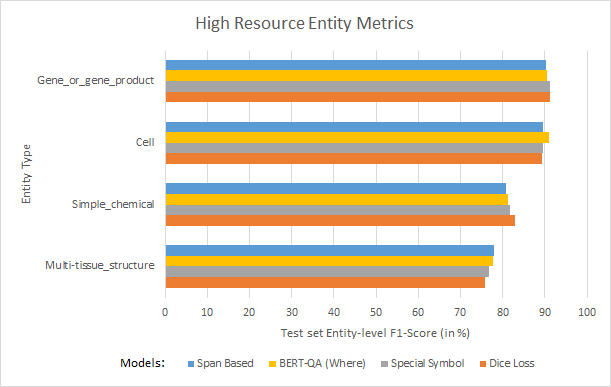
\includegraphics[scale=1.25]{high_resource_entity_metrics}
    \caption{Test set Entity-level F1 scores for high resource entities in \texttt{BioNLP13CG} dataset}
    \label{fig:high_resource_entity_metrics}
\end{figure}

\begin{figure}
    \centering
    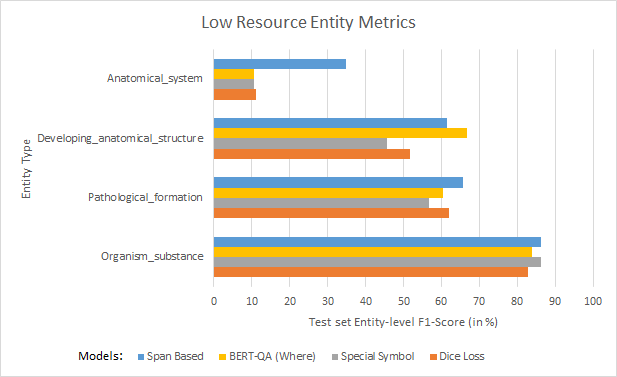
\includegraphics[scale=1.25]{low_resource_entity_metrics}
    \caption{Test set Entity-level F1 scores for low resource entities in \texttt{BioNLP13CG} dataset}
    \label{fig:low_resource_entity_metrics}
\end{figure}

From results in Table \ref{tab:res_macro_f1} and Figures \ref{fig:high_resource_entity_metrics} and \ref{fig:low_resource_entity_metrics}, we make the following observations:
\begin{itemize}
    \item \texttt{Span Based} pipelined approach reports the best overall macro-averaged F1. It is able to perform well even on low-resource entity types. This can be attributed to the span detector which is entity type agnostic and hence does not develop high-resource bias.
    
    \item From overall Macro-F1 scores we see that \texttt{BERT-QA (Where)} and \texttt{Span Based} both use question answering approach internally and perform better than sequence labeling methods. 
    
    \item For high-resource entity types all variants perform comparably while for several low-resource entities, \texttt{Span Based} method takes the lead.
\end{itemize}

\section{Comparison with Other Works}
\label{sec:sota_comparison}
Based on our literature review in the NER domain, we find that different past works differ not only in their approach but also in the data they use and the output entities they focus on. These differences have an impact on the overall performance and make it difficult to have a one-to-one comparison. Hence, in this section we omit a tabular summary and instead give a detailed comparison presenting the results along with the intricacies of each work. 

\subsection{BioNLP13CG}
\cite{crichton2017neural} report $78.90$ as test set micro-F1 in a multi-task learning setup and \cite{neumann2019scispacy} report $77.60$ using their SciSpacy system. BioBERT\cite{lee2020biobert} authors does not state their performance on this dataset however \cite{banerjee2019knowledge} replicate the BioBERT model as a baseline and report $85.56$. Our vanilla BioBERT model achieves $85.99$. \cite{banerjee2019knowledge} report $82.39$ when using the standard train/dev/test splits on their proposed system. When using a combined training corpus of 15 biomedical datasets they get $89.58$, however this setting is not comparable to the other mentioned systems which use only the provided training data. Our \texttt{BERT-QA (Where)} model achieves $86.83$ and \texttt{Span Based} model reports $85.89$ which set the new state-of-the-art on this dataset.

\subsection{CoNLL 2003}
Doing NER on \texttt{CoNLL 2003} data has been a popular NLP task\footnote{https://paperswithcode.com/sota/named-entity-recognition-ner-on-conll-2003} for long. \cite{yamada2020luke} set the current state-of-the-art result at $94.3$ micro-F1 score on test set. They propose a new pretraining task learning entity representations and pretrain the RoBERTa model on a large corpus. Besides, they provide document context as input apart from each sample sentence both during training and inference. BERT\cite{devlin2018bert} reports $92.4$ using a case-preserving WordPiece model including maximal document context available. For each input token, they take the vector representation of the first sub-token and feed to a final classifier. The vector representation is created by concatenating the outputs of top four hidden layers of the BERT transformer. Additionally, as per some discussions on GitHub\footnote{https://github.com/google-research/bert/issues/223}, researchers add additional CRF layer, bidirectional LSTMs along with truecasing and heuristic-based intelligent input sentence splitting as data pre-processing steps to achieve high results. Without these additional steps, the Vanilla BERT-Base model is found to achieve around $91.0$ micro-F1 score. Our experiments with vanilla BERT achieved $91.36$. Using the same vanilla BERT model with our proposed span-based setup, we get $91.64$. Our proposed approach is very generic, simple and efficient. It can be easily combined with popular pre-processing steps described above and custom pre-training done by \cite{yamada2020luke} to further improve the state-of-the-art on this popular dataset.

\subsection{JNLPBA}
From literature review we find that there are two groups into which the past results can be segregated. All figures reported are micro-averaged F1 scores. The first group of works use the version of dataset provided by MTL-Bioinformatics\cite{crichton2017neural} on GitHub\footnote{https://github.com/cambridgeltl/MTL-Bioinformatics-2016/}. For ease of comparison, we also fall into this category. The source paper\cite{crichton2017neural} proposes a multi-task learning setup and reports $70.09$. \cite{wang2019cross} also do multi-task modeling and combine training and development sets of multiple datasets to achieve $73.52$. SciSpacy\cite{neumann2019scispacy} reports $73.21$. \cite{banerjee2019knowledge} report $73.63$ for BioBERT model fine-tuned on JNLPBA. Our vanilla BioBERT setup achieves $74.35$. \cite{sachan2018effective} report $75.03$ using an LSTM-based language model pretraining and fine-tuning procedure. To the best of our knowledge, this work serves as the state-of-the-art on this dataset. Our proposed span-based model reaches $75.01$ which matches with the SOTA.

The second group of papers have parsed and pre-processed the JNLPBA data from scratch. This follows from \cite{yoon2019collabonet} who identified that the MTL-Bioinformatics data version has sentence segmentation issues. \cite{yoon2019collabonet} train on a combined data source consisting of multiple datasets and remove \texttt{Cell\_type} entity class from consideration. They report $78.58$ micro-averaged F1. BioBERT\cite{lee2020biobert} achieves $77.59$. SciBERT\cite{beltagy2019scibert} reports $77.28$ with a CRF used in the final classification step. They mark their results as a macro-F1 score however on cross-referencing with other papers, we suspect it to be a typo which should be micro-F1. Recently \cite{kocaman2021spark} report $81.29$ which serves as a new state-of-the-art in this setting.

We conclude that our proposed span-based architecture gives results equivalent to state-of-the-art on JNLPBA corpus provided on GitHub by MTL-Bioinformatics\cite{crichton2017neural}.
